\chapter*{Questão 4}

\section*{Enunciado}

\noindent
4. Vamos verificar o aumento da entropia e a flecha do tempo no exercício anterior. 
Calcule a entropia como função do número de passos $N$ das moléculas (que é proporcional 
ao tempo $t = N \Delta t$, onde $\Delta t$ é o intervalo de tempo médio entre passos). A entropia é dada por

\begin{equation}
S = - \sum_i P_i \ln P_i,
\end{equation}

\noindent
onde $P_i$ é a probabilidade de se encontrar o sistema em um certo micro-estado $i$. 
Para se definir o micro-estado $i$, definimos um reticulado (muito maior que o tamanho 
de um passo) e verificamos quantas moléculas encontramos em cada célula do reticulado.


\section*{Metodologia}

Nessa simulação é pedido para calcular o valor da entropia de um sistema com \textit{M} 
moléculas, realizando \textit{N} passos. 

Tendo em vista que a entropia do sistema cresce em função do tempo, este que é proporcional 
ao número de passos, $t = N(t-t_0)$, é possível simular o aumento de entropia utilizando 
um aumento no número de passos dados pelas moléculas.

\begin{equation} \label{entropia}
    S = -\sum_{i} P_i \ln{P_i}
\end{equation}

Tendo em vista que a entropia de um sistema é dada pela Equação \ref{entropia}, 
onde $P_i$ é a probabilidade de encontrar o sistema em um certo micro-estado, 
tal que o micro-estado é definido como sendo um reticulado de tamanho fixo 
no qual é medido o número de moléculas que lá estão.

\begin{equation} \label{micro-estado}
    P_i = \frac{K_i}{M}
\end{equation}

Desse modo, através da Equação \ref{micro-estado}, onde $K_i$ é o número de partículas 
no reticulado e $M$ é o número total de moléculas, é possível encontrar a probabilidade 
$P_i$ daquele micro-estado ocorrer.



\section*{Código}

A estrutura principal do código abre um arquivo de saída, percorre 
diferentes valores de $N$ (número de passos) e, para cada caso, chama a função \texttt{calc}, 
que realiza os cálculos necessários para estimar a entropia do sistema.

A função \texttt{calc} é o núcleo do programa. Inicialmente, é definido o tamanho do 
reticulado em função de $N$, bem como os micro-estados disponíveis. Em seguida, o reticulado 
é zerado, e os possíveis passos são definidos como deslocamentos de $\pm 1$ em cada direção. 

A simulação é então realizada para $m$ moléculas, que partem da origem e percorrem $N$ 
passos aleatórios. A cada passo, a direção é escolhida de forma estocástica, com igual 
probabilidade de caminhar no eixo $x$ ou no eixo $y$, e o reticulado registra a posição 
final das partículas.

Após a simulação, a função procede ao cálculo da entropia. O espaço é dividido em regiões 
do reticulado (as células), e conta-se o número de partículas em cada uma. A probabilidade 
$P_i$ de encontrar uma partícula em um micro-estado $i$ é obtida pela razão entre a ocupação 
da célula e o número total de partículas, normalizado pelo fator de discretização. 

Com esses valores, a função aplica a fórmula
\[
S = - \sum_i P_i \ln P_i,
\]
acumulando a contribuição de cada célula do reticulado. 

O valor de entropia calculado é então retornado para o programa principal, que o registra 
no arquivo de saída junto com o respectivo número de passos.


\begin{figure}[h!]
\centering
\caption{Função principal do código.}
\centering
\begin{lstlisting}
program main
        m = 1000
        open(unit=1,file='saida-1-12694394.txt')
        do i = 100,1000
                write(1,7) i,calc(m,i)
        end do
7               format(I12,',',F12.4)
        close(1)
end program main

\end{lstlisting}
\caption*{Fonte: Compilado pelo Autor.}
\label{fig:tarefa 4 - função principal do código}
\end{figure}

\begin{figure}[h!]
\centering
\caption{Função que realiza os cálculos.}
\centering
\begin{lstlisting}
function calc(m,n)
        parameter(iseed=1154)
        dimension ipos(-n:n,-n:n),istep(0:1)
        
        ! Número de micro estados
        irazao = n*0.1
        ! Tamanho do reticulado
        ksize = n/irazao 

        ! Da o seed para o rand()
        rr = rand(iseed)
        ! Inicia o vetor posição
        do i =-n,n
                do j = -n,n
                        ipos(i,j) = 0
                end do
        end do
        
        ! Valores dos passos
        istep(0) = 1
        istep(1) = -1
        

\end{lstlisting}

\caption*{Fonte: Compilado pelo Autor.}
\label{fig:tarefa 4 - função que realiza os cálculos}
\end{figure}




\begin{figure}[h!]
\centering
\caption{Função que realiza os cálculos.}
\centering
\begin{lstlisting}

        ! Realiza os cálculos
        do i = 1,m
                ix = 0
                iy = 0
                do j = 1,n
                idir = 2e0*rand()
                irand = 2e0*rand()

                if (idir .EQ. 0) then
                        ix = ix + istep(irand)
                else
                        iy = iy + istep(irand)
                endif
                end do
                ipos(ix,iy) = ipos(ix,iy) + 1
        end do
        
        ! Calculo reticulado
        calc = 0
        n1 = -n
        n2 = n1 + ksize
        do k =1,2*irazao
                rpro= 0e0

                do i = n1,n2
                        do j = n1,n2
                                rpro = rpro + ipos(i,j) 
                        end do
                end do
                
                rpro = rpro/(irazao)
                
                if (rpro .NE. 0e0) then
                        calc = calc - rpro*log(rpro)

                end if
                ! Muda o valor dos indices
                n1 = n2
                n2 = n2 + ksize
        end do
        return
end function calc
\end{lstlisting}

\caption*{Fonte: Compilado pelo Autor.}
\label{fig:tarefa 4 - função que realiza os cálculos}
\end{figure}

\newpage
\section*{Função calc}


A função calc(m,n) tem por objetivo simular $m$ trajetórias (ou “moléculas”) realizando $n$ passos
cada, registrar a posição final de cada trajetória em um reticulado discreto e, a partir da distribuição
espacial resultante, calcular uma aproximação da entropia de Shannon das probabilidades de
ocupação das células macroscópicas do reticulado. O programa principal chama calc(m,i) para
valores crescentes de $i$ (de 100 a 1000) e grava o par (número de passos, entropia) em arquivo,
permitindo estudar $S$ como função de $N$.

Logo no início da função aparecem definições importantes: parameter (iseed=1154) e dimension ipos(-n:n,-n:n),istep(0:1). O parâmetro iseed é usado para inicializar o gerador de números
pseudo-aleatórios, garantindo reprodutibilidade quando o mesmo iseed for usado sempre; a
chamada rr = rand(iseed) efetua essa semente (dependendo da implementação de rand do
compilador). O array ipos é um contador bidimensional de posições, com índices que vão de $-n$ até
$n$ em cada dimensão — portanto o reticulado fino considerado tem $(2n+1)\times(2n+1)$ células e
pode armazenar posições negativas (o centro da origem é (0,0)). istep(0:1) é reservado para os
incrementos $\pm 1$ que serão aplicados aos deslocamentos em cada passo.

A variável irazao é calculada como n*0.1 (portanto, em termos inteiros, corresponde a 10\% de $n$)
e, segundo o comentário, representa o “número de micro-estados”. Em seguida ksize = n/irazao define o tamanho 
(em células finas) de cada
bloco macroscópico: cada célula macroscópica conterá ksize $\times$ ksize células do reticulado fino. Em
outras palavras, a malha fina (-n:n, -n:n) será agrupada em $2\cdot irazao$ blocos ao longo de cada
dimensão (total de $(2\cdot irazao)^2$ blocos macroscópicos).

A função inicializa ipos com zeros usando dois laços aninhados do tipo do j = -n,n; do i = -n,n. Isso
garante que antes da simulação não haja contagens residuais e que ipos(i,j) passe a ser o
acumulador correto das frequências absolutas de trajetórias que terminaram na posição $(i,j)$.

\begin{figure}[h!]
\centering
\caption{Função principal do código.}
\centering
\begin{lstlisting}
do i = 1,m
    ix = 0
    iy = 0
    do j = 1,n
        idir = 2e0*rand()
        irand = 2e0*rand()
        if (idir .EQ. 0) then
            ix = ix + istep(irand)
        else
            iy = iy + istep(irand)
        endif
    end do
    ipos(ix,iy) = ipos(ix,iy) + 1
end do

\end{lstlisting}

\caption*{Fonte: Compilado pelo Autor.}
\label{fig:tarefa 4 - função que realiza os cálculos}
\end{figure}



Aqui cada trajetória começa em (ix,iy) = (0,0) e executa $n$ passos. As variáveis idir e irand
são usadas para decidir, em cada passo, (i) em qual eixo o passo ocorrerá (x ou y) e (ii) o sinal do passo
(+1 ou -1). Ao atribuir 2.0*rand() (um real entre 0 e 2) a idir e irand, a parte
fracionária é truncada e o valor fica em [0,1] com (aproximadamente) 50\% de chance para cada.
Assim idir=0 seleciona um deslocamento em x, caso contrário em y; irand serve de índice para
istep(irand) onde istep(0)=-1 e istep(1)=1, produzindo passos de unidade para a direita/para
cima ou para a esquerda/para baixo. Ao final dos $n$ passos a posição final (ix,iy) é incrementada
no contador ipos(ix,iy).

Depois de simular $m$ trajetórias, ipos(i,j) contém a frequência absoluta (número de trajetórias)
que terminaram em cada posição do reticulado fino. Para obter a entropia o código soma as contagens ipos em blocos macroscópicos e aplica a fórmula de Shannon. O trecho
relevante é:

\begin{figure}[h!]
\centering
\caption{Função principal do código.}
\centering
\begin{lstlisting}
calc = 0
n1 = -n
n2 = n1 + ksize
do k = 1, 2*irazao
    rpro = 0e0
    do i = n1,n2
        do j = n1,n2
            rpro = rpro + ipos(i,j)
        end do
    end do
    rpro = rpro/(irazao)
    if (rpro .NE. 0e0) then
        calc = calc - rpro*log(rpro)
    end if
    n1 = n2
    n2 = n2 + ksize
end do

\end{lstlisting}

\caption*{Fonte: Compilado pelo Autor.}
\label{fig:tarefa 4 - função que realiza os cálculos}
\end{figure}



Para cada bloco (variando $k$), rpro acumula o número total de trajetórias que caíram nas células
finais pertencentes àquela célula macroscópica. Isso feito, é aplicado a Equação - \ref{entropia}, com o rpro = rpro/(irazao),
que nos da a probabilidade de uma partícula estar no retículado.

\newpage
\section*{Resultados e Discução}

Na Figura - \ref{fig:tarefa 4 - Gráfico entropia versus número de passos}, é apresentado o gráfico gerado
pelo arquivo de saida, é evidente que o acrescésimo no número de passos faz com que a entropia do
sistema aumente.

\begin{figure}[h!]
\centering
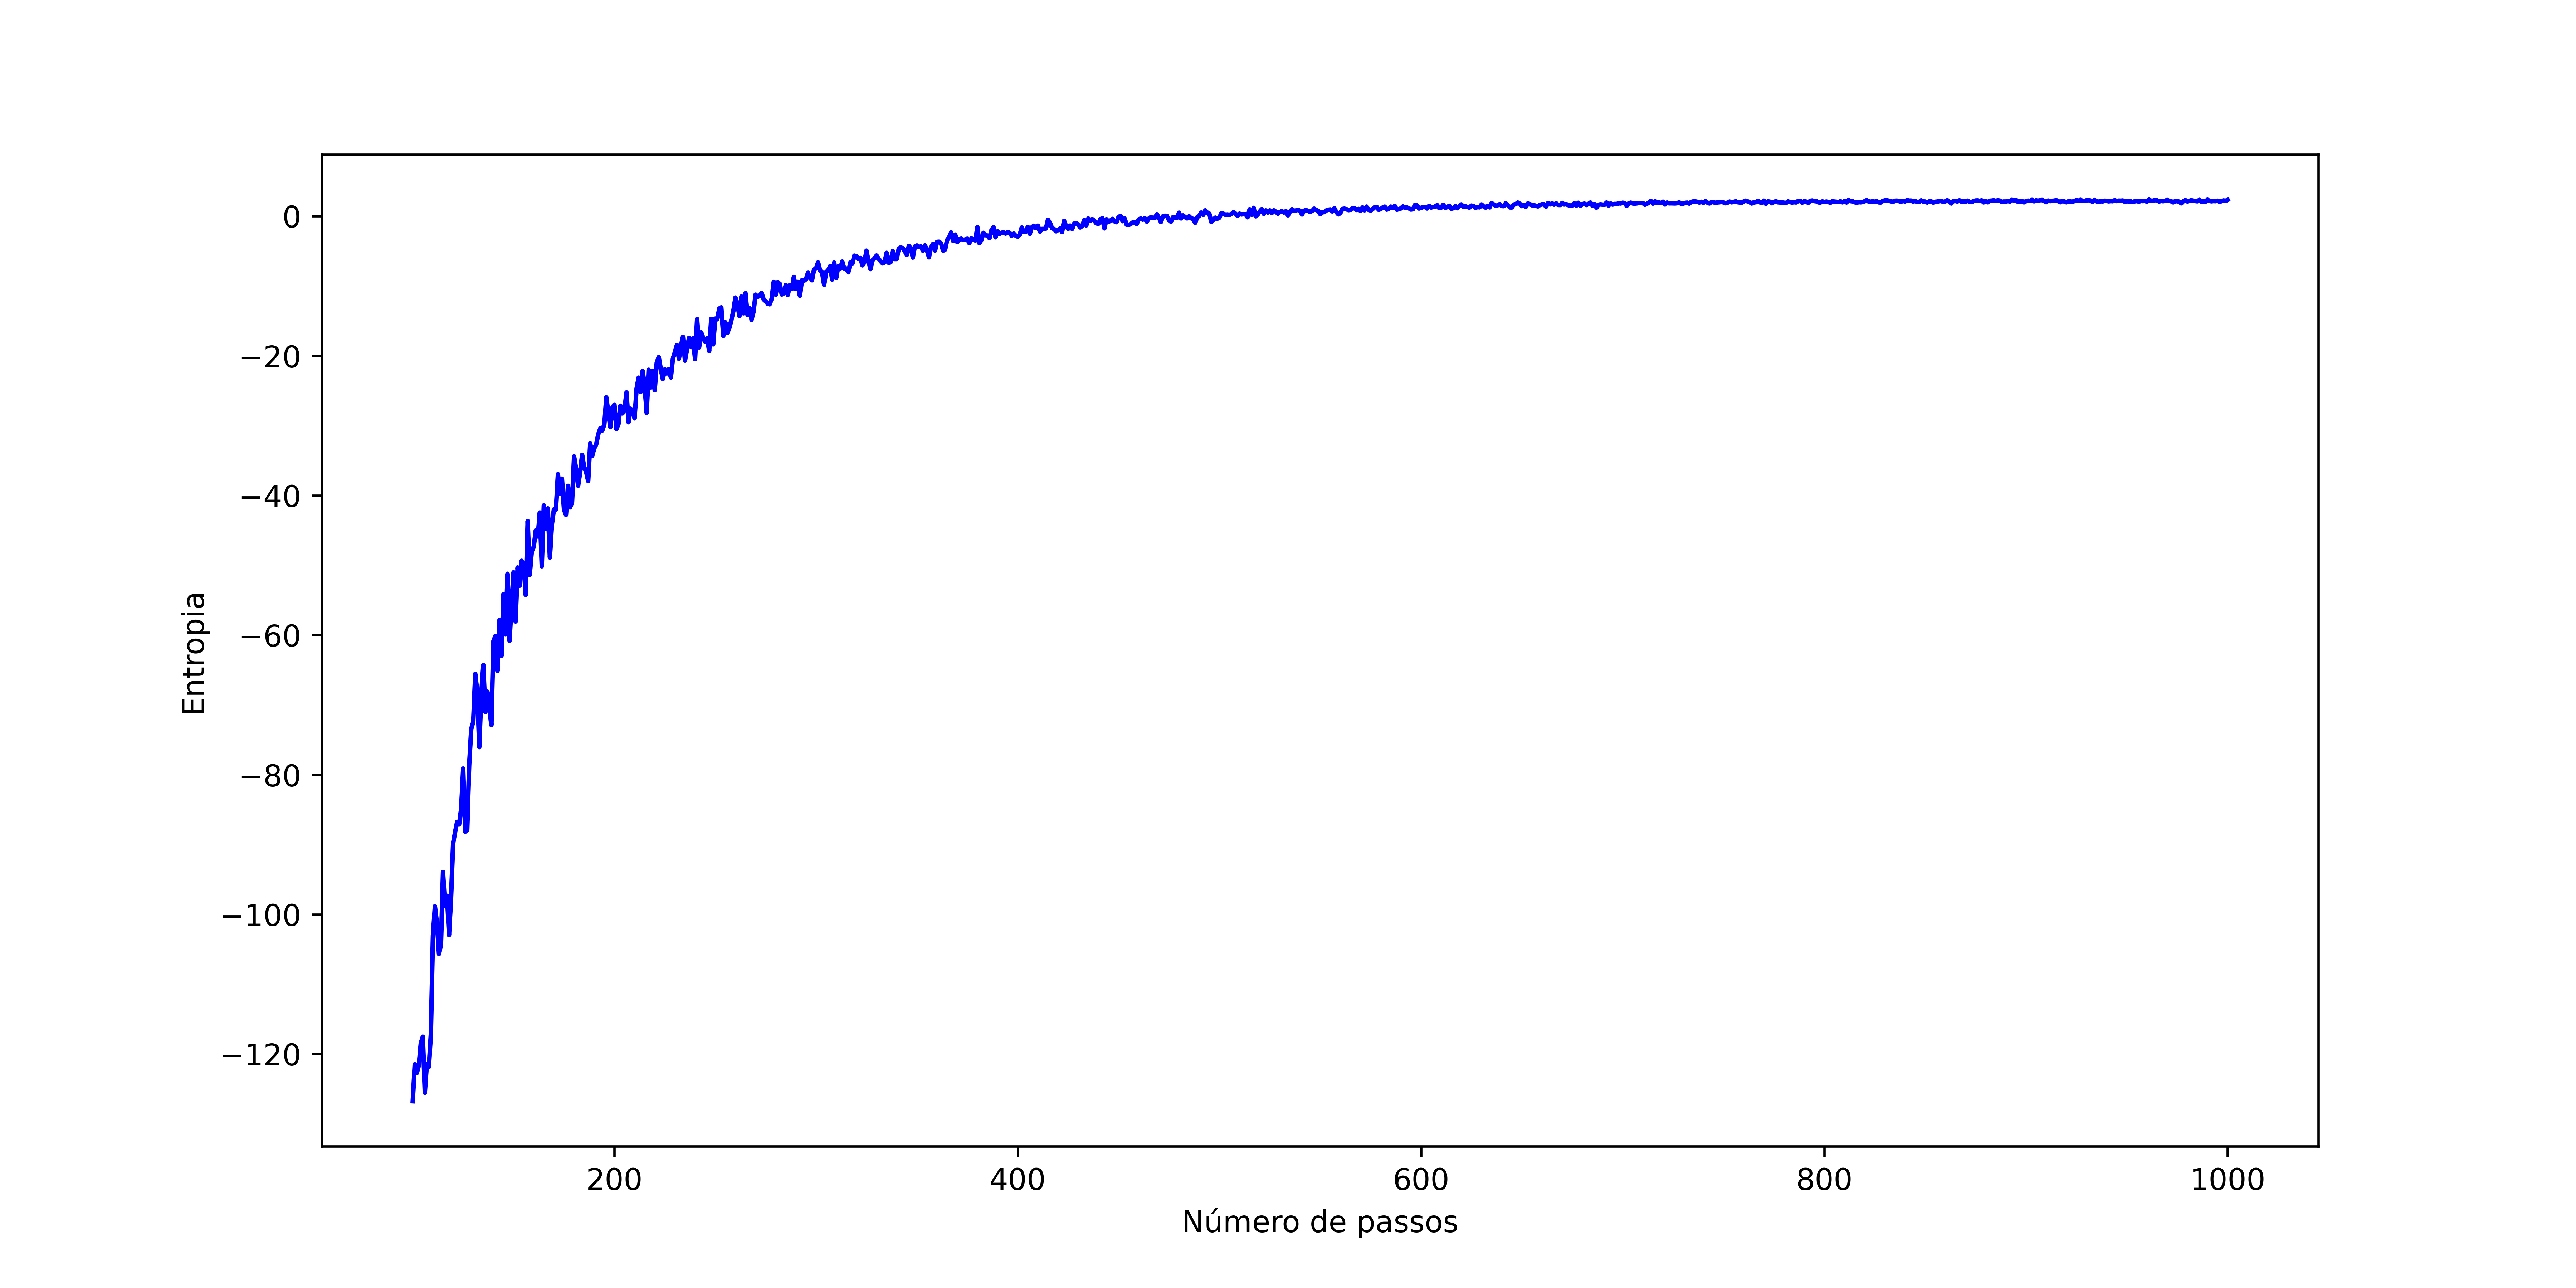
\includegraphics[width=16cm]{images/tarefa-4/tarefa-4-graf-1.png}
\caption{Entropia do sistema vs número de passos}

\caption*{Fonte: Compilado pelo Autor.}
\label{fig:tarefa 4 - Gráfico entropia versus número de passos}
\end{figure}